\documentclass[]{article}
\usepackage{amsmath}\usepackage{amsfonts}
\usepackage[margin=1in,footskip=0.25in]{geometry}
\usepackage{mathtools}
\usepackage{hyperref}
\hypersetup{
    colorlinks=true,
    linkcolor=blue,
    filecolor=magenta,
    urlcolor=cyan,
}
\usepackage[final]{graphicx}
\usepackage{listings}
\usepackage{courier}
\lstset{basicstyle=\footnotesize\ttfamily,breaklines=true}
\newcommand{\indep}{\perp \!\!\! \perp}
% \usepackage{wrapfig}
\graphicspath{{.}}
% \usepackage{fancyvrb}

%%
%% Julia definition (c) 2014 Jubobs
%%
\usepackage[T1]{fontenc}
\usepackage{beramono}
\usepackage[usenames,dvipsnames]{xcolor}
\lstdefinelanguage{Julia}%
  {morekeywords={abstract,break,case,catch,const,continue,do,else,elseif,%
      end,export,false,for,function,immutable,import,importall,if,in,%
      macro,module,otherwise,quote,return,switch,true,try,type,typealias,%
      using,while},%
   sensitive=true,%
   alsoother={$},%
   morecomment=[l]\#,%
   morecomment=[n]{\#=}{=\#},%
   morestring=[s]{"}{"},%
   morestring=[m]{'}{'},%
}[keywords,comments,strings]%

\lstset{%
    language         = Julia,
    basicstyle       = \ttfamily\footnotesize, 
    keywordstyle     = \bfseries\color{blue},
    stringstyle      = \color{magenta},
    commentstyle     = \color{ForestGreen},
    showstringspaces = false,
}
\begin{document}
\begin{center}
    Name: Hongda Li 
    AMATH 585 WINTER 2022 HW5
\end{center}
\section*{The Code}
    The following code is the implementation for both problem 1, 2
    \lstinputlisting{hw5_script.jl}
\section*{Problem 1}
    \subsection*{Theory that goes with the code}
        \hspace{1.1em}
        Natural ordering of the element refers to the mapping of tuple of indices from the grid to the actual point in space, given as $u_{i, j} = u(ih, jh)$. Here, we use equally space point in both xy direction on the unit square: $[0, 1]\times [0, 1]$. And we use $m$ number of interior points, and including the boundary we will have $m + 2$ boundary point. 
        \par
        The implementation focuses on building up the system of matrices using the stencil defined on each point indexed grid point $(i, j)$. For each point, we convert the coordinate indices $(i, j)$ to linear indices for row and column location in the sparse matrix, the coefficient on the stencil is then added to the matrix or the RHS of the system. This is done for $(i, j) \in \{0, 1, \cdots, m\}^2$. If any of the point are laying outside, we move the coefficient to the RHS vector. 
        \par
        Alternatively, one can also use Kronecker Product to construct the structural matrice, but it will lose the elegence of on the code and less generic. Algebraically, one can handle the boundary conditions by thinking about the stencils on the boundary. I only did it for the 5 point stencil. 
        \par
        Let $\mathcal{I}(i, j) = (j - 1)m + i \quad \forall (i, j) \in [1, \cdots, m]\times[1, \cdots m]$ be a mapping from the coordinate indices of the grid point to linear index. Next, we consider partitioning the vector $u$ and $b$ the RHS vector by rows on the grid using natural ordering. 
        \begin{align*}\tag{1.1}\label{eqn:1.1}
            u &= \begin{bmatrix}
                u^{[1]} \\ u^{[2]} \\ \vdots \\ u^{[m]}
            \end{bmatrix}
            \;
            \vec{b} = \begin{bmatrix}
                b^{[1]} \\ b^{[2]} \\ \vdots \\ b^{[m]}
            \end{bmatrix}
            \;
            \vec{f} = \begin{bmatrix}
                f^{[1]} \\ f^{[2]}\\ \vdots \\ f^{[m]}
            \end{bmatrix}
            \\
            u^{[i]} &= 
            \begin{bmatrix}
                u_{1, i} \\ u_{2, i} \\ \vdots \\ u_{m, i}
            \end{bmatrix}
        \end{align*}
        
        \par
        For the bounary conditions, we consider them row by row. Consider the first row: 
        \begin{align*}\tag{1.2}\label{eqn:1.2}
            \begin{aligned}
                \vec{f}_{\mathcal{I}(i, 1)} &= 
                \frac{1}{h^2}
                \text{sum}
                \left(
                    \begin{bmatrix}
                        & u_{i, 2}& 
                        \\
                        u_{i - 1, 1} & -4u_{i, 1}& u_{i + 1, 1}
                        \\
                        & u_{i, 0}& 
                    \end{bmatrix}
                \right) \quad \forall 1 \le i \le m
                \\
                \vec{b}^{[1]} &= 
                - \frac{1}{h^2}\begin{bmatrix}
                    u_{1, 0} \\ u_{2, 0} \\ \vdots \\ u_{m, 0}
                \end{bmatrix}
                - \frac{u_{0, 1}\mathbf{e}_1^{(m)}}{h^2} 
                - \frac{u_{m + 1, 1} \mathbf{e}_{m}^{(m)}}{h^2}
                + f^{[1]}
            \end{aligned}
        \end{align*}
        Next, we consider all the rows in the middle rows: 
        \begin{align*}\tag{1.3}\label{eqn:1.3}
            \begin{aligned}
                \vec{f}_{\mathcal{I}(i, j)} &= 
                \frac{1}{h^2}
                \text{sum}
                \left(
                    \begin{bmatrix}
                        & u_{i, j + 1}& 
                        \\
                        u_{i - 1, j} & -4u_{i, j}& u_{i + 1, j}
                        \\
                        & u_{i, j - 1}& 
                    \end{bmatrix}
                \right) \quad \forall 1 \le i \le m , \; 2 \le j \le m - 1
                \\
                \vec{b}^{[j]} &= 
                - \frac{u_{0, j}\mathbf{e}_{1}^{(m)}}{h^2}
                -
                \frac{u_{m+ 1,j}\mathbf{e}_m^{(m)}}{h^2}
                + f^{[j]}
            \end{aligned}
        \end{align*}
        Finally we consider the last row on the grid point: 
        \begin{align*}\tag{1.4}\label{eqn:1.4}
            \begin{aligned}
                \vec{f}_{\mathcal{I}(i, m)} &= 
                \frac{1}{h^2}\text{sum}
                \left(
                    \begin{bmatrix}
                        & u_{i, m + 1}&  \\
                        u_{i- 1, j}& -4u_{i, m}&  u_{i + 1, j} \\
                        & u_{i, m - 1}&  
                    \end{bmatrix}
                \right)
                \quad \forall\; 1 \le i \le m
                \\
                b^{[m]} &= 
                -\frac{1}{h^2}\begin{bmatrix}
                    u_{1, m + 1} \\ u_{2, m _ 1} \\ \vdots \\ u_{m, m + 1}
                \end{bmatrix} 
                - \frac{u_{0, m}}{h^2}\mathbf{e}^{(m)}_1 
                - \frac{u_{m + 1, m}}{h^2}\mathbf{e}^{(m)}_m
                + \vec{f}^{[m]}
            \end{aligned}
        \end{align*}
        This completes the analysis for the RHS vector that includes the boundary. Take notice that a very different approach has been coded. This part is just for analysis. 
    \subsection*{$\mathcal{O}(h^2)$ Convergence Rate}
        \hspace{1.1em}
        Error computations is made by comparing solution on sparser grid point with the solution obtained on a fine grid point. I don't happen to know the solution of the PDE besides the solution expressed using the Green's function with the given density function.
        \par
        For the implementation of this part, refers to the ``Problem1()'' function. The finer grid is taken with $m = 2^{10} - 1$, and then $m$ follows the pattern of $2^{k} - 1$ so that the discretized grid-point of the sparser grids is a subset of the finer grid. This is a plot of the error measured by $L2$ norm in 2D in log log plot, referenced with $h^2$ convergence: 
        \begin{center}
            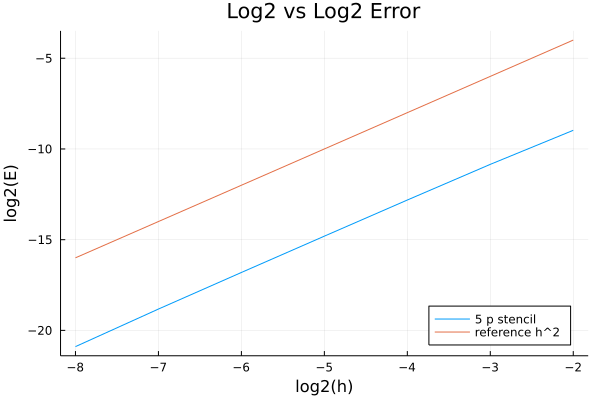
\includegraphics[width=10cm]{p1_fig.png}
        \end{center}
        Numerically, I take the slope of the adjacent points on the log log plot and take the averaging, producing an estimate of the rate of convergence for the 5 points stencil method. The esimated rate is: $1.986773401321141$. 
\section*{Problem 2}
    \hspace{1.1em}
    The same routine is run for the 9-point stencils but with a different definition of the stencil. Deferred correction is implemented by the end, right before the calculation of solution. 
    \par 
    The estimated rate of convergnece of error is $3.0268502045280115$, The error is $\mathcal{O}(n^3)$, which differs from the theory. Here is a plot of the error under log log plot: 
    \begin{center}
        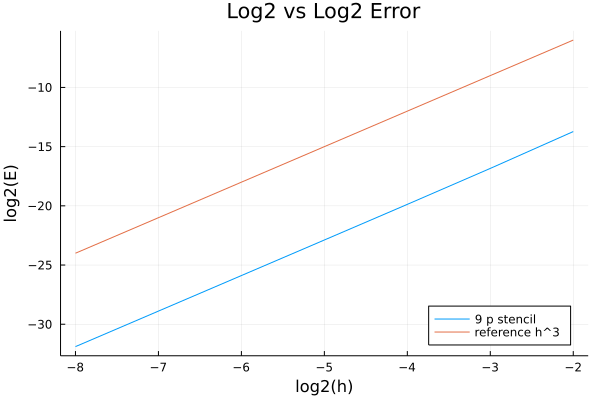
\includegraphics[width=10cm]{p2_fig.png}
    \end{center}
    Observe that this is a mismatch from what is predicted by the theory where it's stated that with deferred correction, the error should have convergence rate of $\mathcal{O}(h^4)$. The cause of the prolem boundary conditions. More specifically, the $\nabla^4[f(x, y)]$ at the boudary point is not defined. Numerially, we have: 
    \begin{align*}\tag{2.1}\label{eqn:2.1}
        \nabla^4[f(x, y)] &= (\partial_x^4 + \partial_y^4 + 2\partial_x^2\partial_y^2)[x^2 + y^2]
        \\
        &= 2 + 2 + 0 = 4 
    \end{align*}
    However, at the boundary point if we assume that the function is $\equiv 1$, then $\nabla^4[u(x, y)]_{(x, y) = \text{bd}([0, 1]^2)} \equiv 0$, making the Laplacian of the RHS function discontinuous at the boundary of the grid, making $\nabla^4[f(x, y)] \neq \nabla^4[u(x, y)]$ at the boundary, failing the assumptions made by the Deferred Correction Method, hence the accuracy of $\mathcal{O}(h^4)$ is not garantee to exists for this particular case.
    \par
    I am not sure why it's $\mathcal{O}(h^3)$ specifically instead of $\mathcal{O}(h^2)$ or anything in between. 

\section*{Problem 3}
    \hspace{1.1em}
    Our goal here is to investigate the format of the System of Linear Equations $(A\vec{c} = \vec{b})$ needed for inhomogenous Poisson Equation on a 2D unit square $\Omega = [0, 1]\times [0, 1]$ with boundary conditions $g(x,y)$ at the boundary. For simplicity of the discussion, we assume the use of gridpoint (Not neccessarily equally spaced) and piecewise bilinear approximation for the problem in $\Omega$. This is the Boundary Value Problem: 
    \begin{align*}\tag{3.1}\label{eqn:3.1}
        \begin{cases}
            \nabla^2\cdot u = f &\forall x \in \Omega
            \\
            u = g & \forall x \in \text{bd}(\Omega)
        \end{cases}
    \end{align*}
    Here we use $\text{bd}(\Omega)$ to denote the boundary of the Domain.
    \par
    Next we consider the weak form and using $S$ as the basis function set: 
    \begin{align*}\tag{3.2}\label{eqn:3.2}
        \forall\; \hat{v}\in S: \langle \mathcal{L}[\hat{u}], \hat{v}\rangle &= \langle 
	    f, \hat{v}
        \rangle
        \\
        \forall\; \hat{v} \in \mathcal{S}:
        \langle \mathcal{L}[\hat{u}], \hat{v}\rangle
        &= 
        \iint_{\Omega}(\hat{u}_{xx} + \hat{u}_{yy})\hat{v}dxdy
        \\
        &= - \iint_{\Omega}(\hat{u}_x\hat{v}_x + \hat{u}_y \hat{v}_y)dxdy 
        +
        \int_{\text{bd}(\Omega)} (\nabla \hat{u})\hat{v} d\hat{\mathbf{n}}
        \\
        &= 
        \int_{\text{bd}(\Omega)} (\nabla u)\hat{v} d\hat{\mathbf{n}} - 
        \iint_{\Omega} (\nabla \hat{u})\cdot (\nabla \hat{v})dxdy
    \end{align*}
    When the set $S$ is finite, we can create a system of equations to assert the conditions presented by the weak form formulation. The definition of inner product is implicitly defined here. 
    \par
    We assume that the grid partitioning $\Omega$ is in the size of $(n_x + 2)\times(n_y + 2)$, including the grid point. $n_x, n_y$ each denotes the number interior discretized grid points on the x, y direction. We use the following notations for mapping coordinate indices on $\Omega$ to linear indices: 
    $$
        \lfloor i, j\rceil = i + 1 + j(n_y + 2)
    $$
    Please observe that $0\le i \le n_x + 1, 0 \le y\le n_y +1$. Now, we are ready to define some set of indices to simplify things: 
    \begin{align*}\tag{3.3}\label{eqn:3.3}
        \begin{aligned}
                \overline{G} &:= \{0, 1, \cdots, n_x + 1\}\times \{0, 1, \cdots, n_y + 1\}
                \\
                G &:= \{1, \cdots, n_x\}\times \{1, \cdots, n_y\}
                \\
                \mathbb{\overline{B}}&:= \overline{G}\setminus G
                \\
                \mathcal{N}(i, j) &:= \{(k, l)\in \overline{G}: |i - k| + |l - j| \le 2\}
            \end{aligned}
    \end{align*}
    The set $\overline{G}$ denotes all the nodes including the nodes at the boundary. And the set $G$ denotesthe nodes that are only inside of the grid, and the set $\overline{\mathbb{B}}$ denotes that set of all the points at the boundary. Finally, the function $\mathcal{N}(i, j)$ dentoes that set of indeices for the nodes that are neighbouring the node at $(i, j)$, including the node that is at $(i, j)$. 
    \par
    In our case, we present the use of Bi-linear Functions on the grid point. Which is paramaterized by 5 points and separated into 5 cases: 
    \begin{equation*}\tag{3.4}\label{eqn:3.4}
        \varphi_{\lfloor i, j \rceil}(x, y)
        = \begin{cases}
            \frac{\left(x-x_{i-1}\right)\left(y-y_{j-1}\right)}{\left(x_{i}-x_{i-1}\right)\left(y_{j}-y_{j-1}\right)} & \text { in }\left[x_{i-1}, x_{i}\right] \times\left[y_{j-1}, y_{j}\right] 
            \\[0.5em]
            \frac{\left(x-x_{i+1}\right)\left(y-y_{j-1}\right)}{\left(x_{i}-x_{i+1}\right)\left(y_{j}-y_{j-1}\right)} & \text { in }\left[x_{i}, x_{i+1}\right] \times\left[y_{j-1}, y_{j}\right] 
            \\[0.5em]
            \frac{\left(x-x_{i-1}\right)\left(y-y_{j+1}\right)}{\left(x_{i}-x_{i-1}\right)\left(y_{j}-y_{j+1}\right)} & \text { in }\left[x_{i-1}, x_{i}\right] \times\left[y_{j}, y_{j+1}\right] 
            \\[0.5em]
            \frac{\left(x-x_{i+1}\right)\left(y-y_{j+1}\right)}{\left(x_{i}-x_{i+1}\right)\left(y_{j}-y_{j+1}\right)} & \text { in }\left[x_{i}, x_{i+1}\right] \times\left[y_{j}, y_{j+1}\right] 
            \\[0.5em]
            0 & \text { elsewhere }
        \end{cases}
    \end{equation*}
    Take notice that, when the function $\varphi$ is at the boundary, for example $\varphi_{\lfloor 0, 0\rceil}$, then it will only have 2 cases instead of 5, because only the top left corner of the square where the node is centered at is defined inside of the grid. By a similar line of reasoning, one can define the bi-linear function for all node with indcies in $\overline{\mathbb{B}}$. Now, we are ready to define that the set of basis functions we use is: $S:= \{\varphi_{\lfloor i,j \rceil}: (i, j)\in \overline{G}\}$. 
    \par
    To make use of the weak Form of Finite Element, we represent the approximated solution $\tilde{u}$ using the set of basis function from $S$: 
    \begin{align*}\tag{3.5}\label{eqn:3.5}
        \tilde{u}(x,y) = 
        \sum_{(i, j)\in \overline{G}}^{}
        c_{\lfloor i,j \rceil}\varphi_{\lfloor i,j \rceil}(x, y)
    \end{align*}
    Before we start, Observe that all the basis functions at the boundary $\text{bd}(\Omega)$ must satisfies the boundary conditions, which immediately gave us $4 + 2(n_x + n_y)$ constraints to work with: 
    \begin{align*}\tag{3.6}\label{eqn:3.6}
        c_{\lfloor i, j\rceil} &= g(x_i, y_j) \quad \forall \; (i, j) \in \overline{\mathbb{B}}
        \\
        \implies
        A_{\lfloor i, j\rceil, \lfloor i, j\rceil} &= 
        1 \quad \forall (i, j) \in \overline{\mathbb{B}}
        \\
        \vec{b}_{\lfloor i,j \rceil} &= g(x_i, y_j)  
        \quad \forall \; (i, j) \in \overline{\mathbb{B}}
    \end{align*}
    \par
    Reconsider the weakform formulations with the given form of approximated solution and the basis set $S$, this will give use constraint for each of the node with indices in $G$, a total of $n_xn_y$ constraints for the system. 
    \begin{align*}\tag{3.7}\label{eqn:3.7}
        \langle \mathcal{L}\tilde{u}, \varphi_{\lfloor i,j \rceil}\rangle &= \langle f, \varphi_{\lfloor i,j \rceil}\rangle \quad \forall \; (i, j) \in G
        \\
        \left\langle 
        \mathcal{L}\left[
            \sum_{(k, l)\in G}^{}
            c_{\lfloor k, l\rceil}\varphi_{
                \lfloor k, l\rceil
            }
            \right], 
            \varphi_{\lfloor i,j \rceil}\right\rangle 
            &= \langle f, \varphi_{\lfloor i,j \rceil}
        \rangle
        \\
        \left\langle 
        \mathcal{L}\left[
            \sum_{(k, l)\in G}^{}
            c_{\lfloor k, l\rceil}\varphi_{
                \lfloor k, l\rceil
            }
            \right], 
            \varphi_{\lfloor i,j \rceil}\right\rangle 
            &= \langle f, \varphi_{\lfloor i,j \rceil}
        \rangle
        \\
        \sum_{(k, l)\in\mathcal{N}(i, j)}^{\forall}c_{\lfloor k, l\rceil}
        \langle \mathcal{L}[\varphi_{\lfloor k,l \rceil}], \varphi_{\lfloor i, j \rceil}\rangle
        &= \langle f, \varphi_{\lfloor i, j \rceil}\rangle
    \end{align*}
    For each of the node with indices in the interior, denoted by $G$, it will interact with all its 8 neighbours, including itself via the dot product defined, and that leads from the second last line to the last line. This gives at most 9 non-zeros element for $n_xn_y$ number of row of the matrix $A$. At this point, we are finally able to present the $(n_x + 2)\times(n_y + 2)$ linear system in a visuall pleasant way: 
    \begin{align*}\tag{3.8}\label{eqn:3.8}
        \forall  (i,j), (k, l) &\in \overline{G}: 
        \\
        A_{\lfloor i,j \rceil, \lfloor k, l \rceil}
        &= 
        \begin{cases}
            \langle \mathcal{L}[\varphi_{\lfloor k, l \rceil}], \varphi_{\lfloor i,j \rceil}\rangle & (k, l) \in \mathcal{N}(i, j)
            \\
            1 & (k, l), (i, j) \in \overline{\mathbb{B}}
            \\
            0 & \text{else}
        \end{cases}
        \\
        \vec{b}_{\lfloor i,j \rceil} &= 
        \begin{cases}
            g(x_i, y_j) & (i, j)\in \overline{\mathbb{B}}
            \\
            \langle f,\varphi_{\lfloor i,j \rceil} \rangle & \text{else}
        \end{cases}
    \end{align*}
    This way of capturing all $(n_x + 2)(n_y + 2)$ number of variables simplifies the right handside of the equation comparing to setting up the $4 + 2(n_x + n_y)$ number of variables for $c_{\lfloor i, j\rceil}$ at the boundary $\overline{\mathbb{B}}$ and then create a system of the size $n_xn_y$ for all the node in $G$. What remains to be evaluated is the inner product between basis function at neighbouring nodes and itself. And recall from \hyperref[eqn:3.2]{(3.2)}, when the one of the nodes at $(i,j)$ or $(k, l)$ is $\in \overline{\mathbb{B}}$, we will have to evaluate an extra integral over the boundary $\text{bd}(\Omega)$. Before we try writing down the entries of the matrix $A$ in integral form, we need to introduce the idea of how non-zeros parts of the basis function intersect with each other and the region $\Omega$ (In this case it's a unit square thankfully). 
    \begin{align*}\tag{3.9}\label{eqn:3.9}
        R((i, j), (k, l)) &= 
        ([x_{\max(i - 1, 0)}, x_{\min(i + 1, n_x + 1)}]\times 
        [y_{\max(j - 1, 0)}, y_{\min(j + 1, n_y + 1)}]) \cdots
        \\
        &\cup 
        (
            [x_{\max(k - 1, 0)}, x_{\min(k + 1, n_x + 1)}]\times
            [y_{\max(l - 1, 0)}, y_{\min(l + 1, n_y + 1)}]
        )
        \\
        \overline{R}(i, j) &= \text{bd}([x_{\max(i - 1, 0)}, x_{\min(i + 1, n_x + 1)}]\times 
        [y_{\max(j - 1, 0)}, y_{\min(j + 1, n_y + 1)}])
    \end{align*}
    $R, \overline{R}$ will programatically represents the non-zero intersection between 2 basis function $\varphi_{\lfloor i,j \rceil}$ and $\varphi_{\lfloor k, l \rceil}$. Therefore, now we can put in a better prepresentation for the inner product in \hyperref[eqn:3.8]{(3.8)} using the weak form of the expression: 
    \begin{align*}\tag{3.10}\label{eqn:3.10}
        & \forall (i, j)\in G \wedge \mathcal{N}(i, j)\cup \overline{\mathbb{B}} = \emptyset: 
        \\
        \langle \varphi_{\lfloor i, j\rceil},\varphi_{\lfloor k, l\rceil}
        \rangle &=
        -\iint_{R((i, j), (k, l))} (\nabla \varphi_{\lfloor i,j \rceil})(\nabla \varphi_{\lfloor k, l\rceil})dxdy
        \\
        & \forall (i, j)\in G \wedge \mathcal{N}(i, j)\cup \overline{\mathbb{B}} \neq \emptyset: 
        \\
        \langle \varphi_{\lfloor i, j\rceil},\varphi_{\lfloor k, l\rceil}
        \rangle &=
        \int_{\text{bd}(\Omega)\cup \overline{R}(i, j)\cup \overline{R}(k, l)}
        (\nabla \varphi_{\lfloor k, l\rceil})\varphi_{\lfloor i, j\rceil}d
        \hat{\mathbf{n}}
        -\iint_{R((i, j), (k, l))} (\nabla \varphi_{\lfloor i,j \rceil})(\nabla \varphi_{\lfloor k, l\rceil})dxdy
    \end{align*}

        

\end{document}